\documentclass[xcolor=dvipsnames]{beamer}
\usepackage{subfig}
\usepackage{wrapfig}
\usetheme{Rochester}  %% Themenwahl
\usecolortheme[named=RoyalBlue]{structure}
\usebackgroundtemplate{
	\centering
	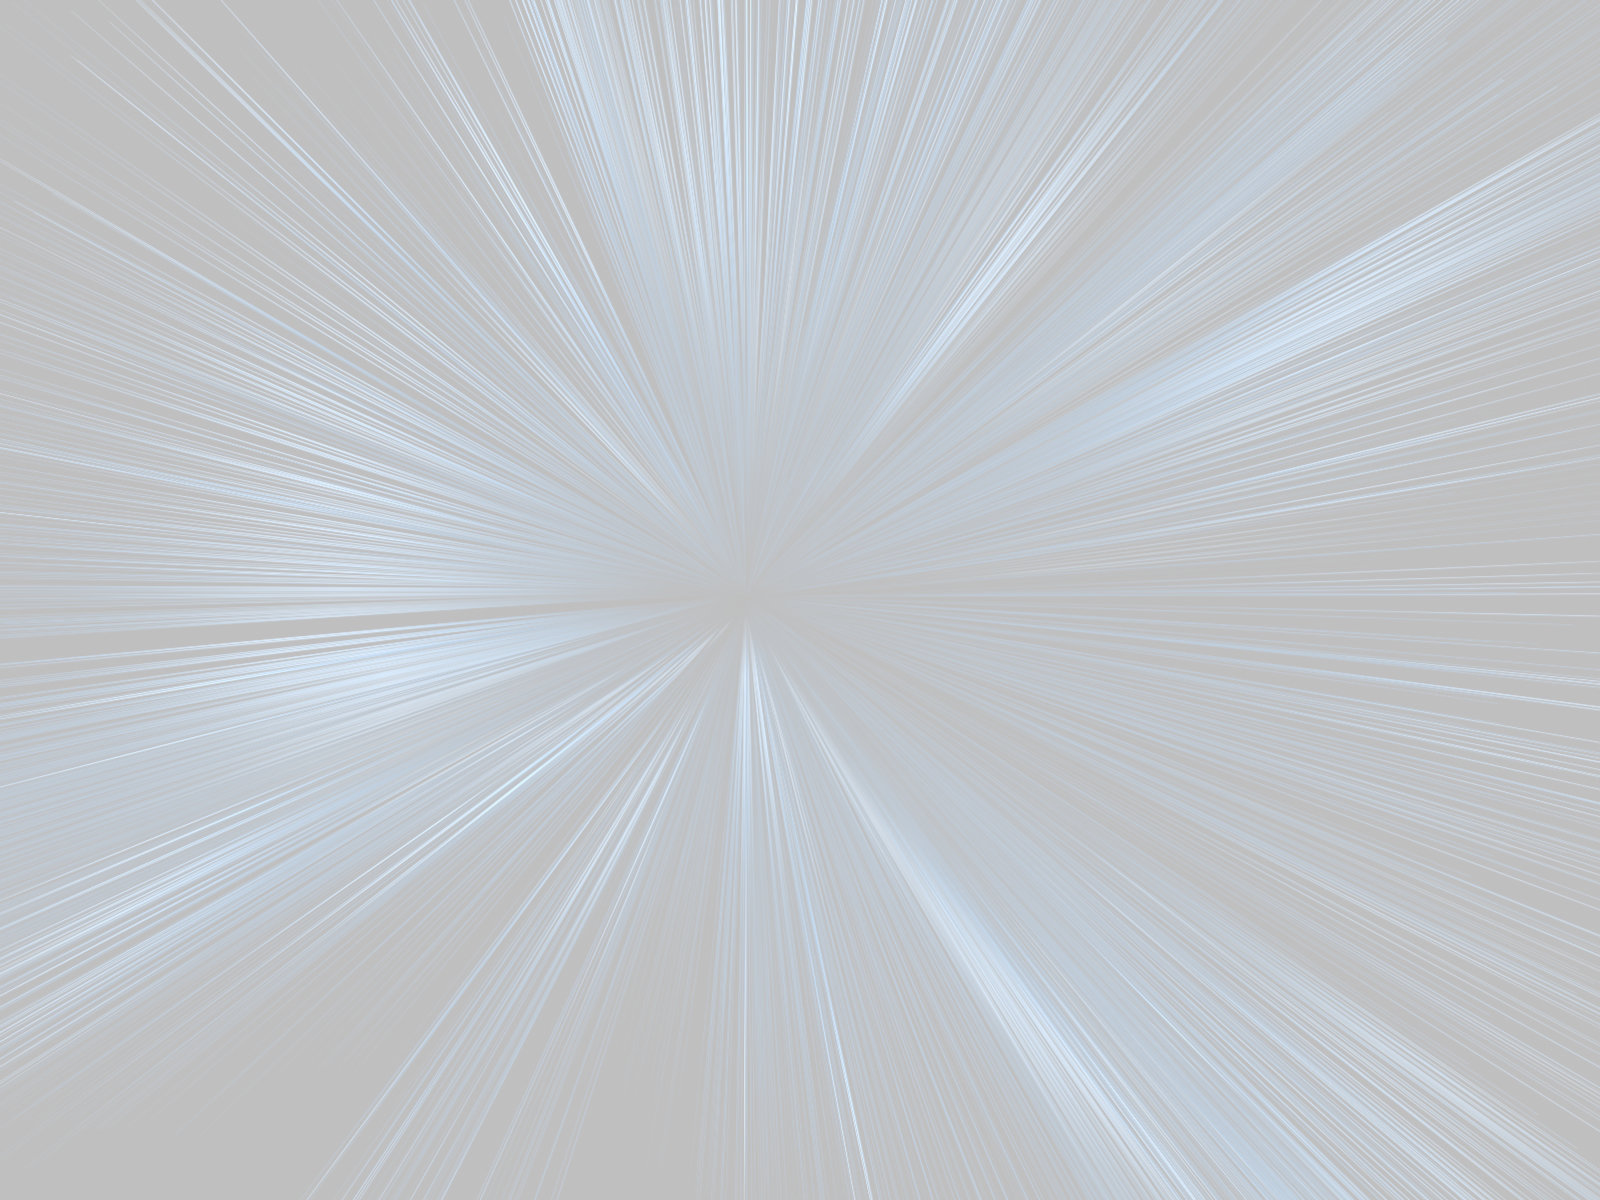
\includegraphics[width=\paperwidth,height=\paperheight]{images/light-speed}
} 

 \addtobeamertemplate{block begin}{\pgfsetfillopacity{0.5}}{\pgfsetfillopacity{1}}
 \addtobeamertemplate{block alerted begin}{\pgfsetfillopacity{0.5}}{\pgfsetfillopacity{1}}
 \addtobeamertemplate{block example begin}{\pgfsetfillopacity{0.5}}{\pgfsetfillopacity{1}}

\setbeamertemplate{navigation symbols}{}

\title{Solve'n Slide}
\subtitle{Playtesting Presentation}
\author{Hanieh Arjomand-Fard\\Kevin Sawischa\\Markus Ansorge\\Stefan Aicher}
\date{10. July 2017}

\begin{document}
	\maketitle
	
	\begin{frame}
		\frametitle{Visual Upgrades}
		\begin{figure}[H]
			\centering
			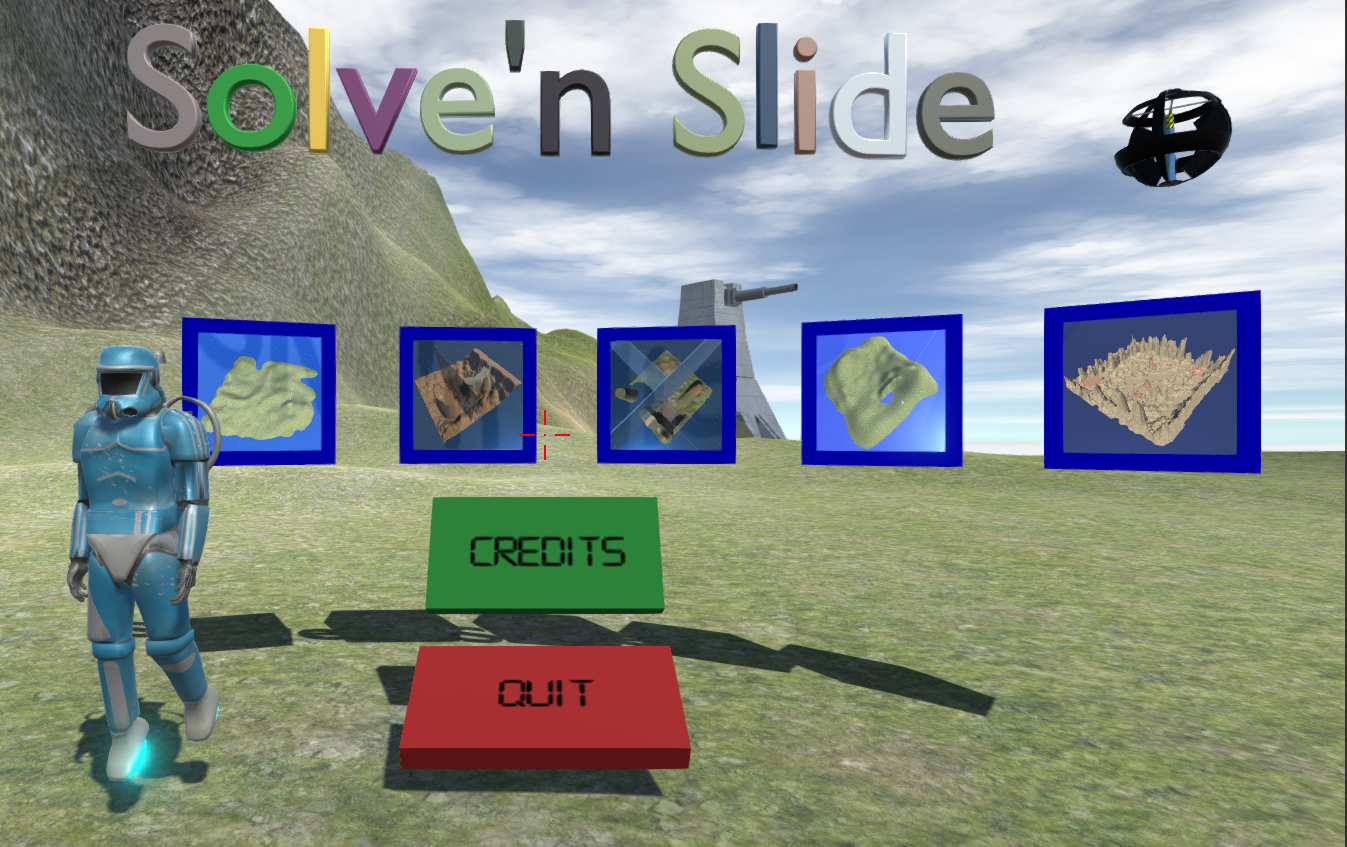
\includegraphics[width=\textwidth]{images/playtesting/MainMenu2}
		\end{figure}
	\end{frame}
	
	\begin{frame}
		\frametitle{Visual Upgrades}
		\begin{figure}[H]
			\centering
			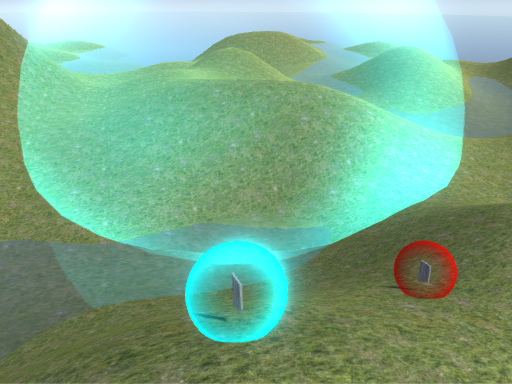
\includegraphics[scale=0.7]{images/playtesting/KeysForceField}
		\end{figure}
	\end{frame}
	
	\begin{frame}
		\frametitle{Testing Procedure}
		\begin{itemize}
			\item 15 participants
			\begin{itemize}
				\item 10 male, 2 female
				\item Age 16 to 27
				\item 12 filled out survey
			\end{itemize}
			\item Testing methodologies
			\begin{itemize}
				\item 7 live tests
				\item 6 Skype tests with screen sharing
				\item 2 Skype tests without screen sharing
			\end{itemize}
			\item Making notes during test
			\item Filling out survey (25 questions) afterwards
		\end{itemize}

		 \begin{figure}[H]
		 	\centering
		 	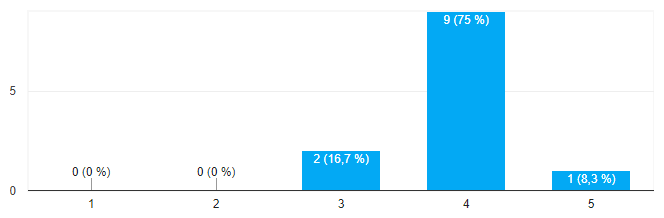
\includegraphics[scale=.4]{images/playtesting/fun}
		 	\caption{How much fun was the game?}
		 \end{figure}
	\end{frame}
	
	\begin{frame}
		\frametitle{Graphics - Main Menu}
		\begin{itemize}
			\item Very controversial
			\item Negative:
			\begin{itemize}
				\item Strange looking level preview images
				\item Option button not working
			\end{itemize}
		\end{itemize}
		\begin{figure}[H]
			\centering
			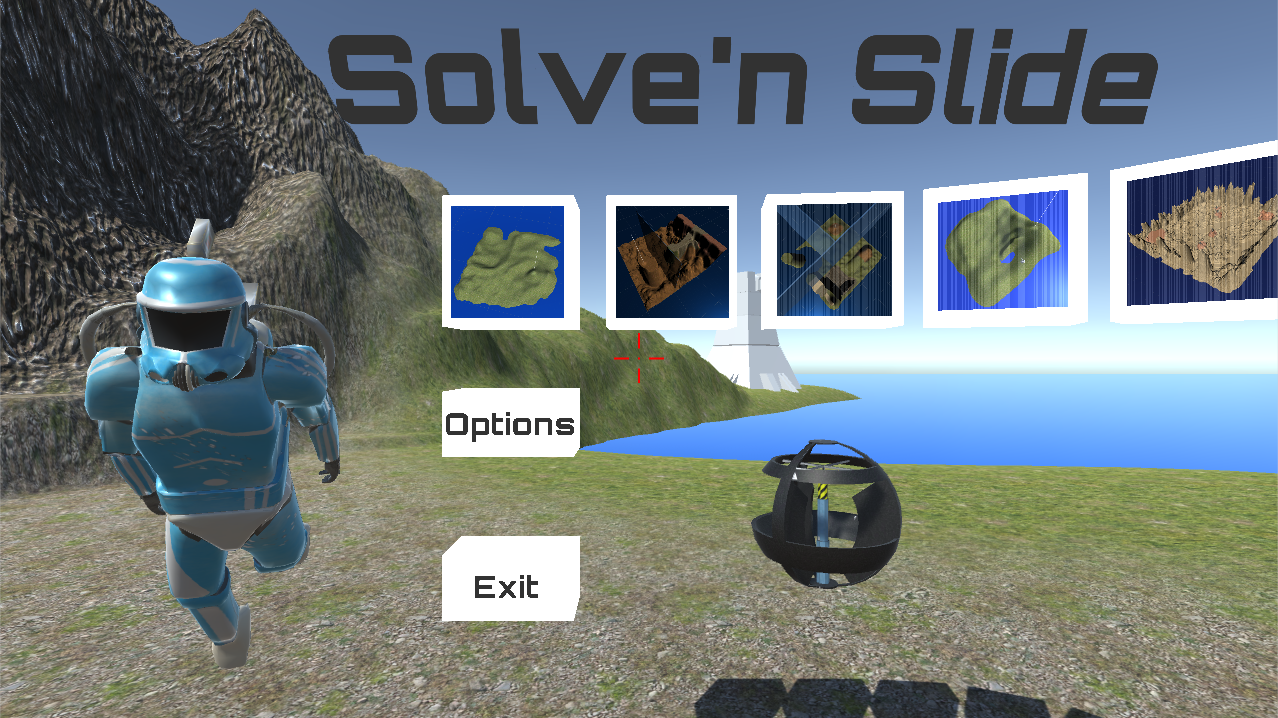
\includegraphics[scale=0.2]{images/playtesting/mainMenu}
		\end{figure}
	\end{frame}
	
	\begin{frame}
		\frametitle{Graphics - User Interface}
		\begin{itemize}
			\item Mostly liked
			\item Negative:
			\begin{itemize}
				\item Inconsistent fuel display between levels
				\item No fuel display in manipulation phase
			\end{itemize}
		\end{itemize}
		\begin{figure}[H]
			\centering
			\begin{tabular}{ccc}
				\subfloat{
\includegraphics[scale=.5]{images/alpha/chargeIcon}}&
				\subfloat{
\includegraphics[scale=.5]{images/alpha/fuelTankIcon}}&
				\subfloat{
\includegraphics[scale=.5]{images/alpha/keyIcon}}
			\end{tabular}
		\end{figure}
		\begin{figure}[ht]
			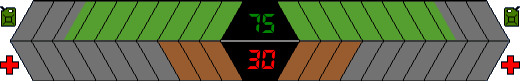
\includegraphics[scale=0.5]{images/alpha/fuelHealthBar}
		\end{figure}
	\end{frame}
	
	\begin{frame}
		\frametitle{Graphics - Environment}
		\begin{itemize}
			\item Most disliked
			\item Negative:
			\begin{itemize}
				\item Terrain looking empty ($\rightarrow$ grass + trees)
				\item Water and forcefields not recognizable ($\rightarrow$ animated textures + shaders)
			\end{itemize}
		\end{itemize}
		\begin{figure}[H]
			\centering
			\begin{tabular}{cc}
				\subfloat{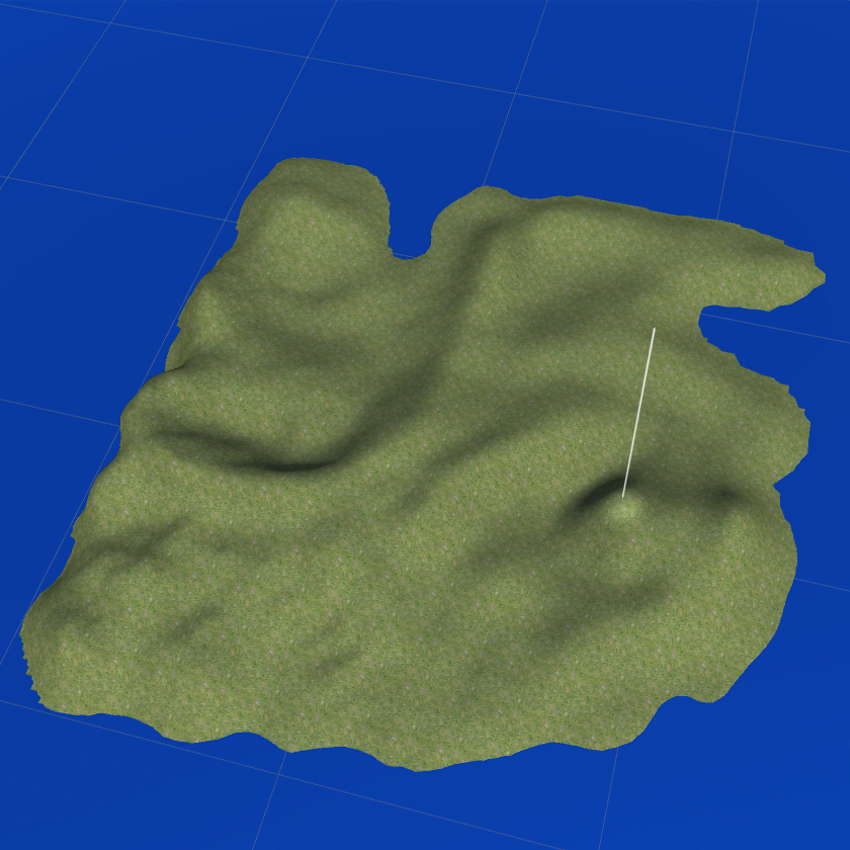
\includegraphics[scale=0.15]{images/playtesting/level1Preview}}&
				\subfloat{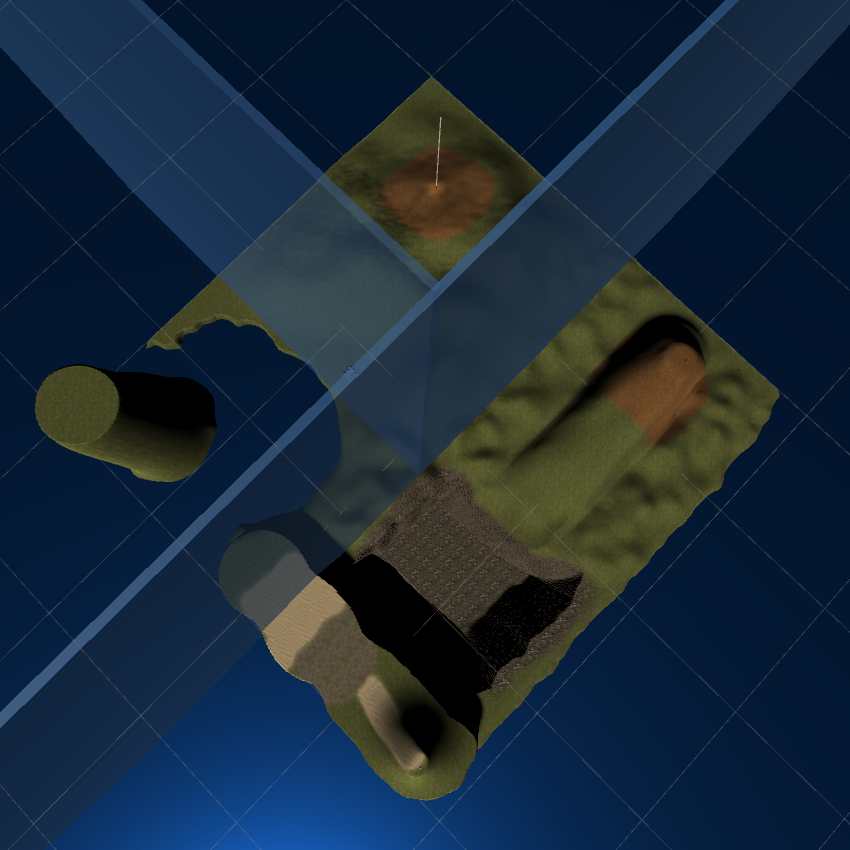
\includegraphics[scale=0.15]{images/playtesting/level3Preview}}
			\end{tabular}
		\end{figure}
	\end{frame}
	
	\begin{frame}
		\frametitle{Controls}
		\begin{itemize}
			\item Biggest criticism: missing information about key bindings
			\item Generally rather intuitive
			\item Changing height with mouse wheel felt strange (prefer combination of shift/ctrl/space)
			\item Dedicated button for restarting action phase needed (e.g. 'R')
		\end{itemize}
		\begin{figure}[ht]
			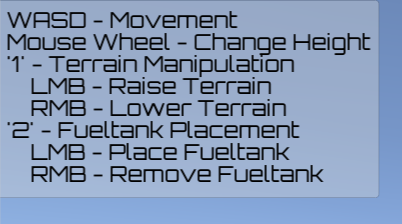
\includegraphics[scale=0.5]{images/playTesting/infoText}
		\end{figure}
	\end{frame}
	
	\begin{frame}
		\frametitle{Gameplay}
		\begin{itemize}
			\setlength\itemsep{2em}
			\item Update function
			\item Crashing
			\begin{itemize}
				\item Screen resolution and graphics
			\end{itemize}
			\item Manipulation phase
			\begin{itemize}
				\item Burying
			\end{itemize}
		\end{itemize}
	\end{frame}
	
	\begin{frame}
		\frametitle{Leveldesign}
		\begin{itemize}
			\setlength\itemsep{2em}
			\item Unclear what to do
			\item Not sure about some objects
			\item Too less of decoration
			\item Too simple
			\item But repetitive
		\end{itemize}
	\end{frame}
	
	\begin{frame}
		\frametitle{Balancing}
		\begin{itemize}
			\setlength\itemsep{2em}
			\item Difficulty
			\item Fix inconsistency
			\item Collision box for fuel tanks and keys
			\item Goal: make fun but still challenging experience
		\end{itemize}
	\end{frame}
	
	\begin{frame}
		\frametitle{Sound Effects}
		\begin{itemize}
			\item Sometimes too loud
			\item In some cases no sound
			\item Wind sound was mistaken for jetpack
		\end{itemize}
	\begin{figure}[ht]
		\centering
		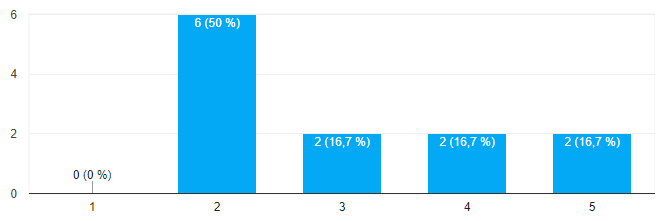
\includegraphics[width=\textwidth]{images/playTesting/sound}
	\end{figure}
	\end{frame}
	
	\begin{frame}
		\frametitle{Wishes and Suggestions}
		\begin{itemize}
			\setlength\itemsep{2em}
			\item Different difficulties
			\item Tutorial
			\item More options
			\item Sound effects
			\item Option/Mode to always place the fuel tank on the ground
		\end{itemize}
	\end{frame}
	
		\begin{frame}
			\frametitle{The End}
			\centering
			\Huge
			Thanks for your attention.
		\end{frame}
\end{document}